% CREATED BY DAVID FRISK, 2016
\chapter{Conclusion}

\section{Discussion}A big portion of inference process for Neural Networks involves massive multiply and add computation, basic operation of tensor convolutions, and across several execution data, especially weight tensors, are reused.
As consequence, for speeding-up and reduce the power consumption (especially in mobile devices) of ML models an hardware accelerator has been developed.
It is also designed for accommodating different data type computation request from Neural Network models, ranging from integer8/16/32/64 to floating-point 32 and brain floating-point 16.\\\\

The approach of the work has been a hardware/software co-design in order to accommodate the high compute intensive request of Machine Learning, the tensor convolution. Therefore, the hardware core for tensor convolution has been developed from scratch, while the common components, such as memories and bus interface, have been chosen from the available ones in the tools.
Moving one step at the time above in the abstraction level, the accelerator library has been developed and deployed. In order to accomplish in a fixed time, the core of the library has been developed in Python, which has been interfaced with a C-code template provided from the developers of thee ML-framework used. This has lead to a hybrid library which encapsulates a frozen Python code layer, called from the C-code, the latter is only in charge of retrieving the data and passing them to the Python layer.
Again one step above in the abstraction, the ML-framework level is reached. In this level, the most popular ML-framework, TensorFlow, has been chosen. It also offers the possibility of delegate part of the execution graph to coprocessor or GPUs. Moreover, Tensorflow pretrained models have been quantized for different bitwidth and data precision.\\\\

It is possible to build a custom hardware accelerator for a specific ML operation and then integrate it into a framework without changing the model nor the framework.
The bottom up approach and the delegate class available in Tensorflow has allowed to fully tailor a new class of hardware accelerators which can accommodate different needs (i.e. depending on which part of the model has to be accelerated). As it has been organized, changing the core software in the Python code and the core in the hardware, it can be also used for addressing different models operations.

\section{Future Works}
For every human artifacts, there is always work to do. In addition, for Computer Engineering artifacts there is also an important step which is the software (and in this case also of the hardware) optimization.
In particular:

\begin{itemize}
\item Software Optimization and migration to a full C code implementation for further reducing the latency.
\item A deep software/hardware testing for finding additional bugs.
\item Power estimation using the simulation’s switching activity in order to obtain a very precise and reliable power consumption.
\item Comparison of model execution on different state-of-the-art platforms.\\
\end{itemize}

Following the previous recommendation, the work may arrive to a competitive level such as the one of the GPUs or other hardware platforms.

\begin{figure}[!htbp]
\centering
\captionsetup{justification=centering}
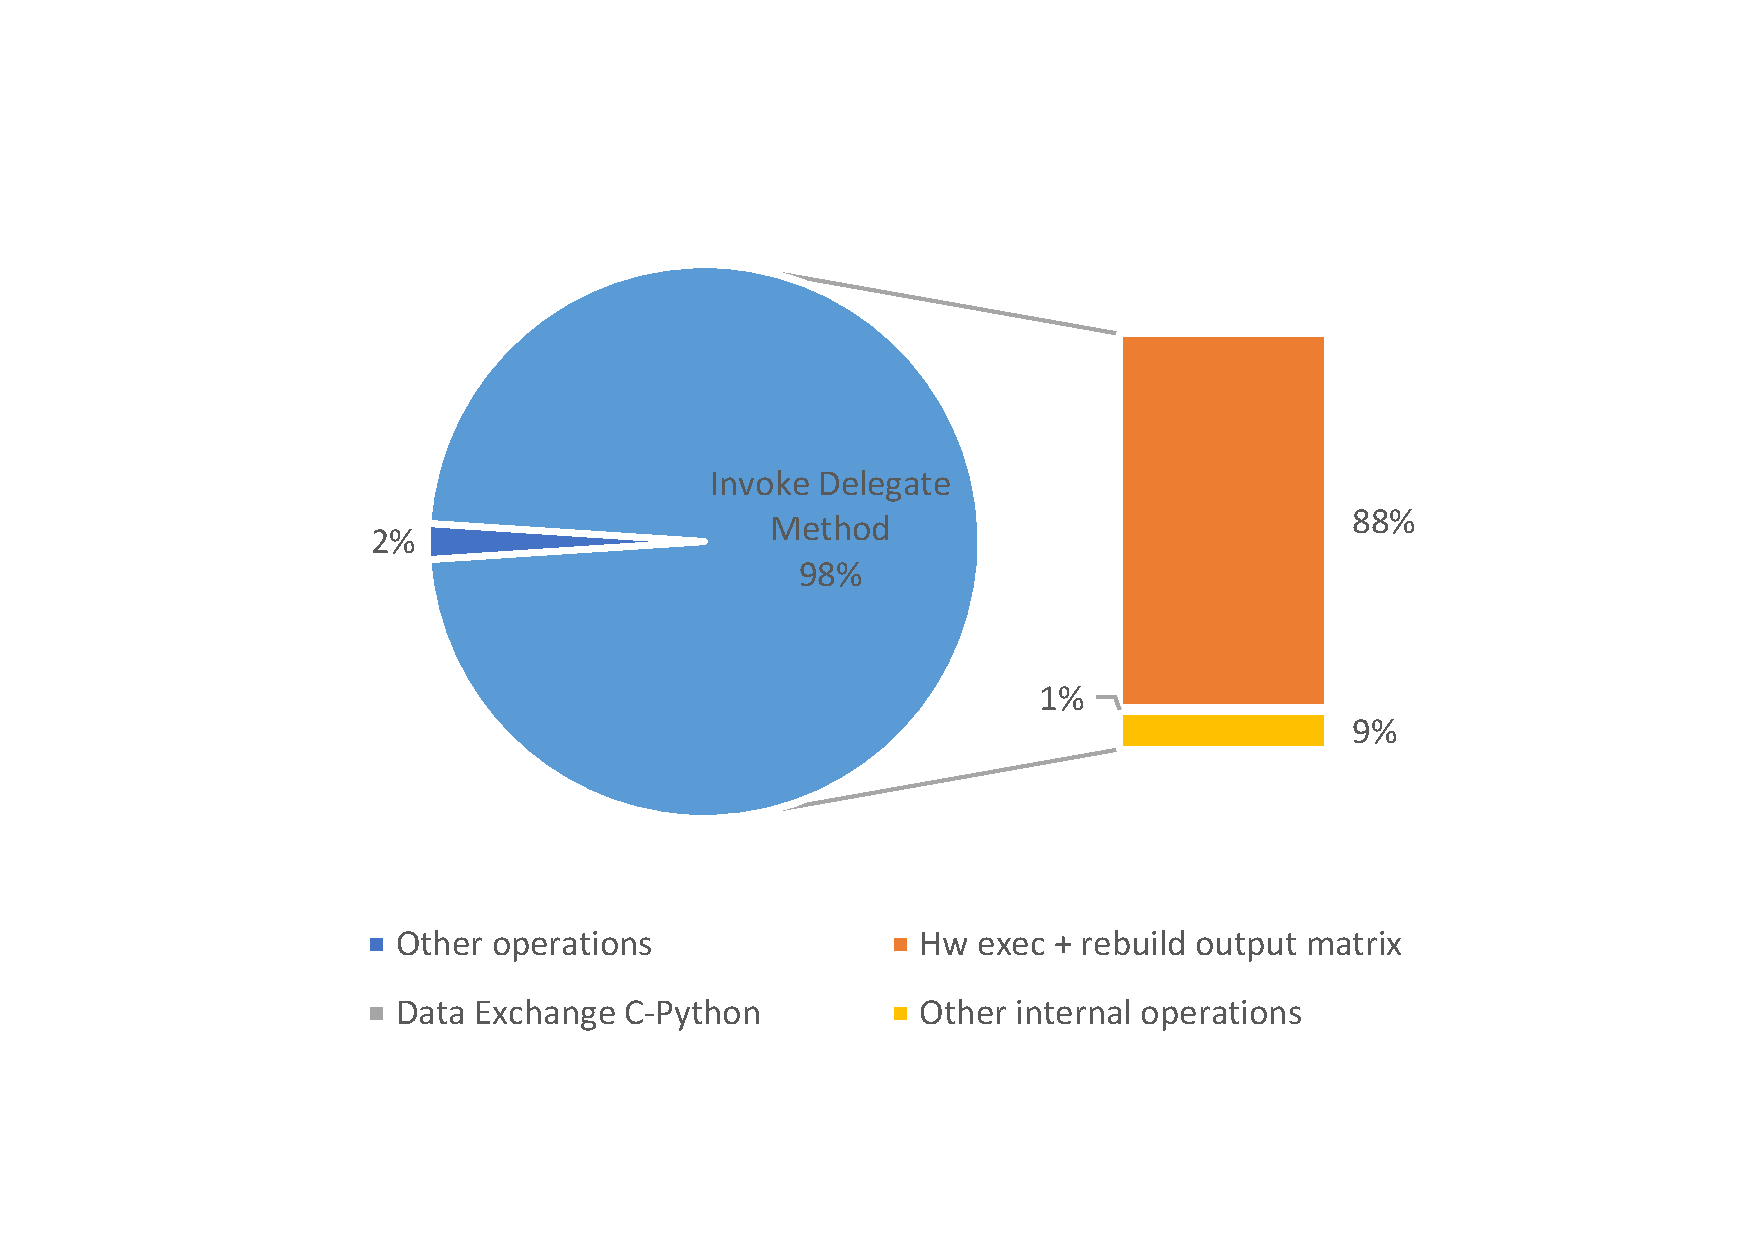
\includegraphics[scale=0.55,angle=0]{./figure/graphs/latency_subdivision_cifar10.pdf}
\caption{Total Execution time of Invoke method (left) in the configuration with accelerator and Cifar10 model}
\label{fig:totexeccifar10}
\end{figure}
\newpage
As it has been mentioned before, the most compute intensive part is always the Convolution operations. Introducing the hardware accelerator and its library comes with several overheads as it can be seen in Figures \ref{fig:totexecmnist} and \ref{fig:totexeccifar10}:\\
\begin{itemize}
\item Data exchange between C and python: the accelerator library has been developed in Python code with the C interface to Tensorflow Lite. This means that every matrix (input, output and weight) is copied to the python sublayer for further processing. Migrating all the accelerator library into C code will remove this overhead.
\item Hardware execution time and rebuilding of output matrix: After every execution of the computation by the accelerator it is parsing the accelerator's output and rebuilding the output matrix accordingly to the current execution indexes. It can be removed preprocessing the model before the deployment, transforming the matrices in a suitable format for the accelerator.
\item Hardware execution time and data transfer to the accelerator: This is the actual execution time of the hardware and the data transfer from/to the accelerator. It is also bounded by the fixed internal memory access. It can be reduced by increasing the frequency of Programmable Logic.
\item Other internal operations: it includes the time for reshaping the input matrix in a format suitable for the accelerator and the save back from python to C of the output matrix. It can be removed preprocessing the model before the deployment, transforming the matrices in a suitable format for the accelerator. Moreover, the migration towards a complete C implementation is going to remove the overhead due to the saving back of the output matrix.\\
\end{itemize}
Taking into account all the previous details and suggestions, the latency of the model can be pushed down to the latency in the solo-CPU execution with the benefits of less power consumption and CPU overload.